
% Appendix A - Vision Document

\chapter{Documento de Visión}
\label{visionDoc}

\section{Propósito}
Ayudar a mejorar los métodos de enseñanza que ofrece la Universidad Técnica Particular de Loja en cuanto a la programación y uso de base de datos para las carreras de Sistemas y Electrónica.
\paragraph{Alcance}
Se propone un sistema de edición de código en línea que a su vez integra LMS externos (para autenticación y notas), un servidor de control de versiones externo (para la persistencia de código), y un servicio web de ejecución de código en línea de una forma segura, eficaz y eficiente (para dar un ambiente de ejecución y pruebas tanto para los usuarios del sistema como para calificar de una forma automática).
\section{Definiciones, Acrónimos y Abreviaciones}
\begin{description}
	\item[LMS] Learning Management System (Sistema de Gestión de Aprendizaje)
    \item[LTI] Learning Tools Interoperability (estandar de Interoperabilidad entre Herramientas de Aprendizaje)
    \item[GitEDU] sistema de Git EDUcation
\end{description}
\subsection{Posición y Oportunidad de Negocios}
Con el avance continuo de la tecnología y su introducción en mas aspectos de la vida diaria, hay una necesidad creciente de ingenieros en sistemas y electrónica que puedan programar y entender el software que hace todo funcionar en adición a las bases de datos que están por detrás de estos mismos sistemas.
 
Es por aquella razón que ahora está de moda ofrecer plataformas en línea para la enseñanza dinámica de la programación. GitEDU espere ofrecer las mismas funcionalidades a un costo institucional menor a través de la integración con sistemas existentes e innovación para proveer una mejor experiencia de usuario, tanto estudiantes como profesores y llevar a cabo un mejor proceso de aprendizaje.

%\pagebreak
%\paragraph{Definición de Problema}
\begin{table}[h!]
  \begin{tabular}{|p{0.2\textwidth}|p{0.7\textwidth}|}
    \hline
    El problema de & enseñar y evaluar programación \\
    \hline
    afecta a & los estudiantes y docentes de las carreras de Sistemas y Electrónica \\
    \hline
    el impacto de lo cual es & el uso ineficiente de recursos universitarios en la enseñanza de la programación \\
    \hline
    Una solución exitosa seria & una aplicación web que ofrezca un editor de código en línea, la capacidad de ejecutar este código para proveer mejor interacción con los estudiantes, la capacidad de ejecutar pruebas unitarias para automatizar el proceso de calificaciones, la persistencia de código en un repositorio de control de versiones remoto para la fácil revisión de profesores y estudiantes, y la integración transparente con sistemas de gestión de aprendizaje externos para la autenticación de usuarios y la respectivo registro de notas. \\
    \hline
  \end{tabular}
  \caption{Definición del Problema.}
  \label{def-prob}
\end{table}

%\pagebreak
%\paragraph{Posición de Producto}
\begin{table}[h!]
  \begin{tabular}{|p{0.2\textwidth}|p{0.7\textwidth}|}
    \hline
    Para & docentes y estudiantes de la Universidad Técnica Particular de Loja \\
    \hline
    Quienes & tienen dificultades en la enseñanza y aprendizaje con la programación \\
    \hline
    GitEDU & es una plataforma web \\
    \hline
    Que & provee un espacio para la interacción entre profesores y alumnos para la enseñanza y aprendizaje de la programación y uso de las bases de datos \\
    \hline
    A diferencia de & otras plataformas altamente costosas que no se integran completamente con sistemas existentes de la universidad ni permiten alta interacción entre docentes y alumnos \\
    \hline
    Nuestro producto & da mayor capacidad para interacción entre estudiantes y sus docentes y se integra bien con las sistemas existentes para dar una mejor experiencia a todos los involucrados a un costo menor. \\
    \hline
  \end{tabular}
  \caption{Posición de Producto.}
  \label{pos-prod}
\end{table}

\pagebreak

\section{Usuarios e Interesados}
\subsection{Demográfica del Mercado}
En el año 2011, la Universidad Técnica Particular de Loja contaba con aproximadamente 4000 estudiantes presenciales y 24000 estudiantes a distancia con una tendencia creciente [UTPL-Datos-Estadisticos]. En la experiencia personal del autor, las carreras de Sistemas y Electrónica, por lo menos en la modalidad presencial, juntos representan aproximadamente un 10\% de todos los estudiantes en la universidad lo cual daría un mercado de estudiantes afectados por un nuevo sistema de aproximadamente un mínimo 2800 estudiantes. Según el directorio de docentes de la universidad, son 60 profesores en el departamento de Ciencias de la Computación y Electrónica [UTPL-Directorio-Docentes]. Con eso se puede estimar un mínimo de 2860 usuarios lo los cuales el sistema propuesto podría llegar a afectar.

Es precisamente la parte de la población, de usuario potenciales mencionado anteriormente, que está en el proceso de enseñar, evaluar y aprender habilidades de programación y consultar bases de datos que forman la base de usuarios de la aplicación.

%\pagebreak
%\paragraph{Resumen de Interesados}
%\begin{table}[h!]
  %\begin{tabular}{|p{0.15\textwidth}|p{0.35\textwidth}|p{0.4\textwidth}|}
% TODO: Caption before longtable, not after %% AESTHETICS
\begin{longtable}{|p{0.2\textwidth}|p{0.35\textwidth}|p{0.35\textwidth}|}
  \hline
  \textbf{Nombre} & \textbf{Descripción} & \textbf{Responsabilidades} \\
  \hline
  \endhead
  Analista & Trabaja con el Asesor Principal y Auxiliar para entender bien las necesidades institucionales para poder llevar un buen ingeniería de requerimientos y diseño del sistema propuesto. & Definir bien el problema para analizarlo, generar requerimientos en base a las necesidades para diseñar y documentar componentes del sistema final para el beneficio del Arquitecto de Software, Programador, Gestor de Proyecto y futuro mano de obra en el proyecto. \\
  \hline
  Arquitecto de Software & Trabaja con el Asesor Principal y Auxiliar para definir una arquitectura que garantiza que se cumpla con los atributos de calidad que requiere el sistema y será compatible con la infraestructura y sistemas institucionales ya existentes. & Diseñar los modelos de interacción entre todos los componentes internos y externos del sistema para con ello lograr un flujo eficaz y eficiente, que también cumple con los parámetros de los requerimientos no funcionales, en el sistema final. \\
  \hline
  Gestor de Proyecto & Trabaja con el Asesor Principal y Auxiliar para evaluar, estimar y establecer el alcance, los recursos y el cronograma del proyecto. & Distribuir de manera eficiente y eficaz los recursos para ayudar el analista, arquitecto de software, programador y administrador de sistemas y bases de datos cumplir dentro de los recursos, alcance y cronograma preestablecido. \\
  \hline
  Programador & Trabaja con el Asesor Principal, Asesor Auxiliar, y Analista para implementar soluciones técnicas que cumplen con el diseño dado por el analista. & Desarrollar el sistema en todos sus componentes. \\
  \hline
  Administrador de Sistemas y Bases de Datos & Trabaja con el Asesor Principal y Auxiliar para desplegar la aplicación en la institución. & El despliegue correcto del sistema con todos sus componentes en la institución respectivo. \\
  \hline
  Asesor Principal & Trabaja con el Asesor Auxiliar para poder aconsejar de la mejor manera el Analista, Arquitecto de Software, Gestor de Proyecto, Programador y Administrador de Sistemas y Bases de Datos. & La definición de necesidades y aprobación del producto final. \\
  \hline
  Asesor Auxiliar & Trabaja con el Asesor Principal para poder aconsejar de la mejor manera al Analista, Arquitecto de Software, Gestor de Proyecto, Programador y Administrador de Sistemas y Bases de Datos. & La definición de necesidades y aprobación del producto final. \\
  \hline
  Asesor de Documentación & Trabaja con el Analista y Gestor de Proyecto para asegurar la calidad de la documentación que se genera a lo largo del proyecto y que se cumple con el cronograma establecido entre el gestor del proyecto y los asesores principales y auxiliares. & La aprobación de los avances en la documentación y la documentación completa al final del proyecto. \\
  \hline
  %\end{tabular}
  \caption{Resumen de Interesados.}
  \label{res-inter}
\end{longtable}
%\end{table}

%\pagebreak
%\paragraph{Posición de Producto}
\begin{table}[h!]
  \begin{tabular}{|p{0.225\textwidth}|p{0.225\textwidth}|p{0.225\textwidth}|p{0.225\textwidth}|}
    \hline
    \textbf{Nombre} & \textbf{Descripción} & \textbf{Responsabilidades} & \textbf{Interesado} \\
    \hline
    Estudiantes & Usuario final primario del sistema & Usa la aplicación para cumplir con las tareas, pruebas y exámenes que propone el docente & Los mismos \\
    \hline
    Professores & Usuario final primario del sistema & Usa la aplicación para ingresar tareas, pruebas y exámenes a los estudiantes y calificar los mismos & Los mismos \\
    \hline
    Administradores & Quienes administran el sistema en su ambiente de despliegue & Mantener el sistema & El mismo \\
    \hline
  \end{tabular}
  \caption{Resumen de Usuarios.}
  \label{res-user}
\end{table}

\subsection{Ambiente de Usuario}
El sistema será disponible para el uso de los usuarios que estén en el campus universitario y en sus hogares.

\subsection{Perfiles de Interesados}
Para entender a fondo cada clase de interesado, a continuacion se presenta un análisis de los mismos.

\pagebreak

%\textbf{Analista}
%\pagebreak
\begin{table}[h!]
  \begin{tabular}{|p{0.45\textwidth}|p{0.45\textwidth}|}
    \hline
    \textbf{Descripción} & El analista del equipo de desarrollo \\
    \hline
    \textbf{Tipo} & Miembro del Equipo de Desarrollo \\
    \hline
    \textbf{Responsabilidades} & Definir bien el problema para analizarlo, generar requerimientos en base a las necesidades para diseñar y documentar componentes del sistema final para el beneficio del Arquitecto de Software, Programador, Gestor de Proyecto y futuro mano de obra en el proyecto. \\
    \hline
    \textbf{Criterio de éxito} & Llevaar a cabo exitosamente el proyecto bajo todos sus requerimientos funcionales y no funcionales \\
    \hline
    \textbf{Involucramiento} & En cada fase del proyecto \\
    \hline
    \textbf{Entregables} & Documentación del sistema y su funcionamiento \\
    \hline
    \textbf{Comentarios / Preocupaciones} & Que se cumpla con todas las necesidades institucionales \\
    \hline
  \end{tabular}
  \caption{Perfil de Interesado: Analista.}
  \label{per-inter-analista}
\end{table}

\vfill

%\textbf{Arquitecto de Software}
%\pagebreak
\begin{table}[h!]
  \begin{tabular}{|p{0.45\textwidth}|p{0.45\textwidth}|}
    \hline
    \textbf{Descripción} & El arquitecto de software en el equipo de desarrollo \\
    \hline
    \textbf{Tipo} & Miembro del Equipo de Desarrollo \\
    \hline
    \textbf{Responsabilidades} & Diseñar los modelos de interacción entre todos los componentes internos y externos del sistema para con ello lograr un flujo eficaz y eficiente, que también cumple con los parámetros de los requerimientos no funcionales, en el sistema final. \\
    \hline
    \textbf{Criteroa de éxito} & Que se lleve a cabo exitosamente el proyecto bajo todos sus requerimientos no funcionales \\
    \hline
    \textbf{Involucramiento} & En cada fase del diseño y despliegue \\
    \hline
    \textbf{Entregables} & Modelos Arquitectónicos del Sistema y su interacción con otros sistemas \\
    \hline
    \textbf{Comentarios / Preocupaciones} & Que cumpla con todas las atributos de calidad que la institución manda \\
    \hline
  \end{tabular}
  \caption{Perfil de Interesado: Arquitecto de Software.}
  \label{per-inter-arquitecto}
\end{table}

\pagebreak

%\textbf{Gestor de Proyecto}
%\pagebreak
\begin{table}[h!]
  \begin{tabular}{|p{0.45\textwidth}|p{0.45\textwidth}|}
    \hline
    \textbf{Descripción} & El gestor de proyecto en el equipo de desarrollo \\
    \hline
    \textbf{Tipo} & Miembro del Equipo de Desarrollo \\
    \hline
    \textbf{Responsabilidades} & Distribuir de manera eficiente y eficaz los recursos para ayudar el analista, arquitecto de software, programador y administrador de sistemas y bases de datos cumplir dentro de los recursos, alcance y cronograma preestablecido. \\
    \hline
    \textbf{Criterio de éxito} & Que se lleve a cabo exitosamente el proyecto bajo todos sus requerimientos y dentro de los recursos y cronograma preestablecido. \\
    \hline
    \textbf{Involucramiento} & En cada fase del proyecto \\
    \hline
    \textbf{Entregables} & Documentación de la gestión del proyecto y el adecuado seguimiento y control interno a lo largo del mismo \\
    \hline
    \textbf{Comentarios / Preocupaciones} & Que se cumpla con todo el proyecto dentro de los recursos y cronograma preestablecido \\
    \hline
  \end{tabular}
  \caption{Perfil de Interesado: Gestor de Proyecto.}
  \label{per-inter-project-manager}
\end{table}

\vfill

%\textbf{Programador}
%\pagebreak
\begin{table}[h!]
  \begin{tabular}{|p{0.45\textwidth}|p{0.45\textwidth}|}
    \hline
    \textbf{Descripción} & El programador del equipo de desarrollo \\
    \hline
    \textbf{Tipo} & Miembro del Equipo de Desarrollo \\
    \hline
    \textbf{Responsabilidades} & Desarrollar el sistema en todos sus componentes. \\
    \hline
    \textbf{Criterio de éxito} & Que se lleve a cabo exitosamente el proyecto bajo todos sus requerimientos funcionales y no funcionales \\
    \hline
    \textbf{Involucramiento} & En cada fase del desarrollo del proyecto \\
    \hline
    \textbf{Entregables} & Código del Sistema \\
    \hline
    \textbf{Comentarios / Preocupaciones} & Que se logra programar segun la especificación que el analista le da \\
    \hline
  \end{tabular}
  \caption{Perfil de Interesado: Programador.}
  \label{per-inter-programer}
\end{table}

\pagebreak

%\textbf{Administrador de Sistemas y Bases de Datos}
%\pagebreak
\begin{table}[h!]
  \begin{tabular}{|p{0.45\textwidth}|p{0.45\textwidth}|}
    \hline
    \textbf{Descripción} & El administrador de sistemas y bases de datos del equipo de desarrollo \\
    \hline
    \textbf{Tipo} & Miembro del Equipo de Desarrollo \\
    \hline
    \textbf{Responsabilidades} & El despliegue correcto del sistema con todos sus componentes en la institución respectiva. \\
    \hline
    \textbf{Criterio de éxito} & Que se lleve a cabo exitosamente el proyecto bajo todos sus requerimientos funcionales y no funcionales \\
    \hline
    \textbf{Involucramiento} & En cada fase del desarrollo y despliegue del proyecto \\
    \hline
    \textbf{Entregables} & Documentación de los Servicios Desplegados \\
    \hline
    \textbf{Comentarios / Preocupaciones} & Que se logre desplegar la aplicación según la especificación del arquitecto de software \\
    \hline
  \end{tabular}
  \caption{Perfil de Interesado: Administrador de Sistemas y Bases de Datos.}
  \label{per-inter-admn}
\end{table}

\vfill

%\textbf{Asesor Principal}
%\pagebreak
\begin{table}[h!]
  \begin{tabular}{|p{0.45\textwidth}|p{0.45\textwidth}|}
    \hline
    \textbf{Descripción} & El asesor principal para equipo de desarrollo \\
    \hline
    \textbf{Tipo} & Asesor del Equipo de Desarrollo \\
    \hline
    \textbf{Responsabilidades} & La definición de necesidades y aprobación del producto final. \\
    \hline
    \textbf{Criteria de Exito} & La entrega del producto final \\
    \hline
    \textbf{Involucramiento} & En cada fase del proyecto \\
    \hline
    \textbf{Entregables} & Aprobación del Producto Final \\
    \hline
    \textbf{Comentarios / Preocupaciones} & Que se logra realizar la aplicación. \\
    \hline
  \end{tabular}
  \caption{Perfil de Interesado: Asesor Principal.}
  \label{per-inter-a-prin}
\end{table}

\vfill

%\textbf{Asesor Auxiliar}
%\pagebreak
\begin{table}[h!]
  \begin{tabular}{|p{0.45\textwidth}|p{0.45\textwidth}|}
    \hline
    \textbf{Descripción} & El asesor auxiliar para equipo de desarrollo \\
    \hline
    \textbf{Tipo} & Asesor del Equipo de Desarrollo \\
    \hline
    \textbf{Responsabilidades} & La definición de necesidades y aprobación del producto final. \\
    \hline
    \textbf{Criterio de éxito} & La entrega del producto final \\
    \hline
    \textbf{Involucramiento} & En cada fase del proyecto \\
    \hline
    \textbf{Entregables} & Aprobación del producto final \\
    \hline
    \textbf{Comentarios / Preocupaciones} & Que se logre realizar la aplicación. \\
    \hline
  \end{tabular}
  \caption{Perfil de Interesado: Asesor Auxiliar.}
  \label{per-inter-a-aux}
\end{table}

\pagebreak

%\textbf{Asesor de Documentación}
%\pagebreak
\begin{table}[h!]
  \begin{tabular}{|p{0.45\textwidth}|p{0.45\textwidth}|}
    \hline
    \textbf{Descripción} & El asesor de documentación para equipo de desarrollo \\
    \hline
    \textbf{Tipo} & Asesor del Equipo de Desarrollo \\
    \hline
    \textbf{Responsabilidades} & La aprobación de los avances en la documentación y la documentación completa al final del proyecto. \\
    \hline
    \textbf{Criterio de éxito} & La entrega de la documentación final \\
    \hline
    \textbf{Involucramiento} & En cada fase del proyecto \\
    \hline
    \textbf{Entregables} & Aprobación de la Documentación Final y los respectivos avances \\
    \hline
    \textbf{Comentarios / Preocupaciones} & Que se logre realizar la documentación. \\


















template

Autenticación inteligente para estudiantes de evaluación en linea


Autenticación inteligente para estudiantes de evaluación en linea


Autenticación inteligente para estudiantes de evaluación en linea
    \hline
  \end{tabular}
  \caption{Perfil de Interesado: Asesor de Documentación.}
  \label{per-inter-a-doc}
\end{table}

%%%%%%%%%%%%%%%%%%%%%%%%%%%%%
\vfill

\subsection{Perfiles de Usuarios}
Para entender a fondo cada clase de usuario se da a continuación un analisis de los mismos.

%\textbf{Estudiante}
%\pagebreak
\begin{table}[h!]
  \begin{tabular}{|p{0.45\textwidth}|p{0.45\textwidth}|}
    \hline
    \textbf{Descripción} & Estudiantes de la Modalidad Presencial y a Distancia de las carreras de Sistemas y Electrónica \\
    \hline
    \textbf{Tipo} & Usuario Final Primario \\
    \hline
    \textbf{Responsabilidades} & Probar el sistema \\
    \hline
    \textbf{Criterio de éxito} & Que el sistema sea de utilidad para su experiencia educativa \\
    \hline
    \textbf{Involucramiento} & En la fase de pruebas \\
    \hline
    \textbf{Entregables} & Ninguno \\
    \hline
    \textbf{Comentarios / Preocupaciones} & Que la aplicación sea fácil de usar \\
    \hline
  \end{tabular}
  \caption{Perfil de Usuario: Estudiante.}
  \label{per-user-estu}
\end{table}

%\textbf{Professor}
%\pagebreak
\begin{table}[h!]
  \begin{tabular}{|p{0.45\textwidth}|p{0.45\textwidth}|}
    \hline
    \textbf{Descripción} & Profesores de Programación y de Bases de Datos de la Modalidad Presencial y a Distancia de las carreras de Sistemas y Electrónica \\
    \hline
    \textbf{Tipo} & Usuario final primario \\
    \hline
    \textbf{Responsabilidades} & Probar el sistema \\
    \hline
    \textbf{Criterio de éxito} & Que el sistema sea de utilidad para su docencia \\
    \hline
    \textbf{Involucramiento} & En la fase de pruebas \\
    \hline
    \textbf{Entregables} & Ninguno \\
    \hline
    \textbf{Comentarios / Preocupaciones} & Que la aplicación les facilite el proceso de enseñanza \\
    \hline
  \end{tabular}
  \caption{Perfil de Usuario: Profesor.}
  \label{per-user-prof}
\end{table}

\pagebreak

%\textbf{Administrador}
%\pagebreak
\begin{table}[h!]
  \begin{tabular}{|p{0.45\textwidth}|p{0.45\textwidth}|}
    \hline
    \textbf{Descripción} & Administradores Institucionales de Sistemas y de Bases de Datos \\
    \hline
    \textbf{Tipo} & Usuario final secundario \\
    \hline
    \textbf{Responsabilidades} & Mantener el Sistema \\
    \hline
    \textbf{Criteria de Exito} & Que el sistema sea fácil de mantener \\
    \hline
    \textbf{Involucramiento} & En las fases de pruebas y despliegue \\
    \hline
    \textbf{Entregables} & Ninguno \\
    \hline
    \textbf{Comentarios / Preocupaciones} & Que la aplicación sea lo suficientemente documentado \\
    \hline
  \end{tabular}
  \caption{Perfil de Usuario: Administrador.}
  \label{per-user-admn}
\end{table}

\subsection{Necesidades de Interesados y Usuarios Principales}
En base a los interesados y usuarios principales definidos, se define las necesidades del sistema a continuacion.

%\begin{table}[h!]
%	\begin{tabular}{|p{0.13\textwidth}|p{0.13\textwidth}|p{0.20\textwidth}|p{0.14\textwidth}|p{0.20\textwidth}|}
% TODO: Caption before longtable, not after %% AESTHETICS
\begin{longtable}{|p{0.13\textwidth}|p{0.13\textwidth}|p{0.20\textwidth}|p{0.14\textwidth}|p{0.20\textwidth}|}
		\hline
        \textbf{Necesidad} & \textbf{Prioridad} & \textbf{Preocupaciones} & \textbf{Solución Seleccionado} & \textbf{Soluciones Propuestas} \\
        \hline
        \endhead
        Seguridad en el Ambiente de Ejecución de Código & Alta & Las partes del sistema que se encargan de ejecución de código, necesitan alta protección contra usuario maliciosos y daños accidentales. & Ver las soluciones propuestas & Virtualización:	
        	\begin{itemize}
        		\item \small{Hipervisor de Tipo 1}
                \item Hipervisor de Tipo 2
                \item Contener-ización
        	\end{itemize}
            \\
        \hline
        Extensi-bilidad & Alta & El sistema debe soportar funcionalidades agregadas en el futuro. & Aplicación orientada a la Modularidad, ver la solución propuesta para mayor detalle. & Modularidad entre componentes del sistema para facilitar el proceso de agregar componentes nuevos o reemplazar componentes existentes sin tocar los demás \\
        \hline
        Facilidad en Autenticación & Mediana & El sistema debe ser fácil para autenticar todos sus usuarios. & Autentica-ción contra LMS existente mediante LTI & Autenticación contra LMS existente mediante LTI \\
        \hline
        Facilidad en Notas & Mediana & El sistema debe ser capaz de registrar notas en sistemas externas sin interacción del profesor. & Registro de Notas mediante LTI & Registro de Notas mediante LTI \\
        \hline
        Facilidad en Persistencia de Código & Mediana & El sistema, sin necesidad de interacción del usuario debe persistir el código escrito en un servidor de algún sistema de control de versiones externa & Transferencia de código mediante sistemas de control de versiones ya existentes & Transferencia de código mediante sistemas de control de versiones ya existentes \\
        \hline        
%	\end{tabular}
	\caption{Necesidades de Interesados y Usuarios Principales}
    \label{nec-inter-user}
%\end{table}
\end{longtable}

\subsection{Alternativas y Competidores}
\begin{enumerate}
	\item Repl.it
    \item Cloud9 IDE
\end{enumerate}

\pagebreak

\section{Vista General de Producto}
\subsection{Perspectiva del Producto}
\begin{figure}[h!]
  \begin{center}
  	% TODO: Bigger? %% AESTHETICS
    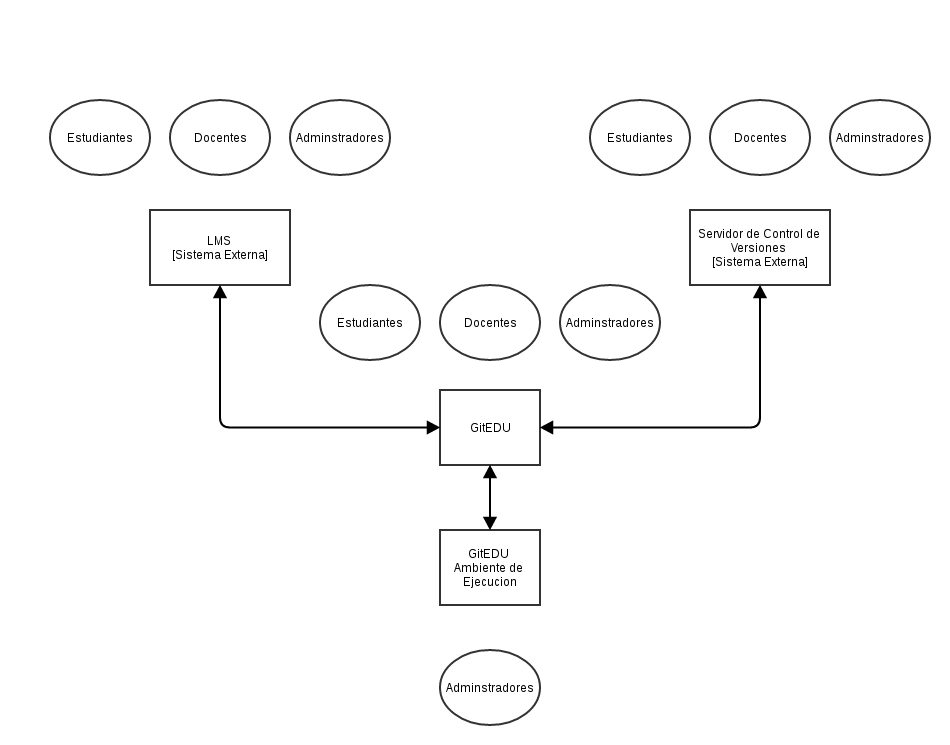
\includegraphics[width=0.75\textwidth]{Figures/pers-prod.png}
  \end{center}
  \caption{Perspectiva del Producto.}
  \label{pers-prod}
\end{figure}

%\pagebreak

\subsection{Resumen de Capacidades}
\begin{table}[h!]
  \begin{tabular}{|p{0.45\textwidth}|p{0.45\textwidth}|}
    \hline
    \textbf{Beneficio al Cliente} & \textbf{Característica de Apoyo} \\
    \hline
    Facilidad de autenticación & Autenticación por LTI contra LMS institucional \\
    \hline
    Gestión de la configuración para el código escrito & Uso de servidores externos de control de versiones \\
    \hline
    Ejecución y pruebas uunitarias en línea & sistema de apoyo con ambiente de ejecución de código \\
    \hline
    Generación y sincronización de notas & calificación a través de pruebas unitarias, sincronización de notas a través de LTI con LMS institucional \\
    \hline
  \end{tabular}
  \caption{Resumen de Capacidades.}
  \label{res-cap}
\end{table}

\subsection{Presuposiciones y Dependencias}
\begin{enumerate}
	\item La institución seguirá usando Moodle y Open EDX como sus plataformas y proveedores de LMS.
	\item La institución seguirá usando como proveedor de un servidor de control de versiones de la institución, un servidor institucional con GitLab Community Edition.
	\item Alternativas como Repl.it y Cloud9 IDE no dan la funcionalidad necesaria o son demasiados costosos para su uso general por la institución.
\end{enumerate}

%\pagebreak

\section{Caracteristicas de Producto}
\begin{enumerate}
	\item Caracteristicas de Autenticación
    	\begin{enumerate}
			\item Autenticarse por LTI
			\item Autenticarse con Usuario y Contraseña
			\item Cerrar Session   
    	\end{enumerate}
    
	\item Caracteristicas de Editar Código
    	\begin{enumerate}
			\item Nuevo Proyecto
			\item Nuevo Proyecto basado en otro Proyecto
			\item Ver Proyectos
			\item Ver Detalles de un Proyecto
			\item Editar Detalles de un Proyecto
			\item Gestionar Usuarios de un Proyecto
			\item Gestionar Permisos de un Proyecto
			\item Abrir Proyecto
			\item Editar Archivos en un Proyecto
			\item Crear Nuevo Archivo en un Proyecto
			\item Borrar Archivo de un Proyecto
			\item Interactuar con Usuarios dentro de un Proyecto
    	\end{enumerate}
    
	\item Caracteristicas de Persistencia de Codigo
    	\begin{enumerate}
			\item Guardar cambios en un Proyecto
			\item Subir cambios en un Proyecto
			\item Bajar cambios en un Proyecto
    	\end{enumerate}
	\item Caracteristicas de Ejecutar y Calificar Código
    	\begin{enumerate}
			\item Ejecutar Codigo en ambiente interactivo en el navegador
			\item Agregar Pruebas Unitarias a un Proyecto
			\item Ejecutar Pruebas Unitarias en un Proyecto
			\item Calificar un Proyecto
			\item Calificiar un Proyecto de forma Automática en base a Pruebas Unitarias
			\item Enviar Calificaciones a un Sistema Externo
    	\end{enumerate}
\end{enumerate}

\pagebreak

\section{Precedencia y Prioridades}
\begin{table}[h!]
  \begin{tabular}{|p{0.45\textwidth}|p{0.45\textwidth}|}
    \hline
    \textbf{Prioridad} & \textbf{Característica (Según su número)} \\
    \hline
    Alta & 1.a, 1.c, 2.a, 2.b, 2.c, 2.h, 2.i, 3.a, 3.b, 4.a \\
    \hline
    Media & 1.b, 2.f, 2.g, 2.j, 3.c, 4.b, 4.c, 4.d, 4.f \\
    \hline
    Baja & 2.d, 2.e, 2.k, 2.l, 4.e \\
    \hline
  \end{tabular}
  \caption{Precedencia y Prioridades.}
  \label{precedencia-y-prioridades}
\end{table}

\section{Restricciones}
\subsection{Seguridad}
Protección contra ataques en la red

Aislamiento de ambientes de ejecución de código de usuarios
\subsection{Extensibilidad}
Soporte al nivel de sistema y documentación para extensión con más lenguajes de programación y motores de base de datos al futuro
\subsection{Usabilidad}
Ser usable

Requerir un mínimo de interacción del usuario para que puede enfocarse en realizar sus responsabilidades en el sistema
\subsection{Escalabilidad}
Tener capacidad para escalar frente mayor carga en el futuro
\subsection{Rendimiento}
Minimizar las requerimientos mínimos de hardware requerido
\section{Otros Requisitos de Producto}
\subsection{Normas}
Ninguna.
\subsection{Requisitos de Sistema}
Ninguno.
\subsection{Requisitos de Rendimiento}
Ninguno.
\subsection{Requisitos Ambientales}
Ninguno.
\section{Requisitos de Documentación}
\subsection{Manual del Programador}
Documentación para explicar el funcionamiento de la aplicación para que futuros desarrolladores puedan extender sin mayor dificultad la aplicación.
\subsection{Manual de Mantenimiento}
Documentación para definir los procesos de mantenimiento de la aplicación para guiar la gobernanza y administración del mismo.
\subsection{Manual de Usuario}
Documentación para enseñar el uso de la aplicación a docentes y alumnos.

